% Requires only \usepackage{tikz}.  The figure is native vector artwork.
\begin{figure}[t]
\centering
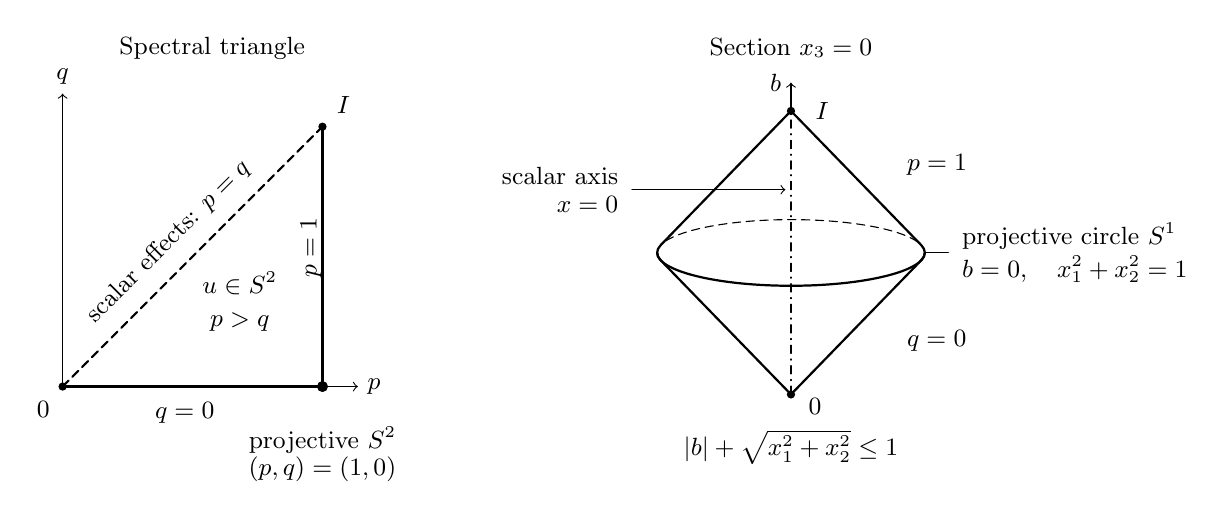
\begin{tikzpicture}[x=1cm,y=1cm,line cap=round,line join=round,
                    font=\small]
  % Left panel: exact ordered spectral triangle.
  \node at (1.9,4.30) {Spectral triangle};
  \draw[->,thin] (0,0) -- (3.75,0) node[right] {$p$};
  \draw[->,thin] (0,0) -- (0,3.72) node[above] {$q$};
  \draw[thick] (0,0) -- (3.3,0) -- (3.3,3.3);
  \draw[thick,densely dashed] (0,0) -- (3.3,3.3);
  \node[rotate=45,anchor=south] at (1.53,1.65)
    {scalar effects: $p=q$};
  \node[anchor=north] at (1.55,-0.08) {$q=0$};
  \node[rotate=90,anchor=south] at (3.41,1.77) {$p=1$};
  \node[align=center] at (2.25,1.08) {$u\in S^2$\\[1pt]$p>q$};
  \fill (0,0) circle (1.5pt);
  \fill (3.3,3.3) circle (1.5pt);
  \fill (3.3,0) circle (2pt);
  \node[anchor=north east] at (-0.04,-0.06) {$0$};
  \node[anchor=south west] at (3.36,3.34) {$I$};
  \node[anchor=north,align=center] at (3.30,-0.39)
    {projective $S^2$\\[-1pt]$(p,q)=(1,0)$};

  % Right panel: a three-dimensional section, shown in linear projection.
  % In local coordinates the map is
  % (x_1,x_2,b) -> (1.70*x_1,0.42*x_2+1.80*b).
  % The cone silhouette meets the projected unit circle at its exact
  % tangency points: sin(alpha)=0.42/1.80=7/30.
  \begin{scope}[shift={(9.25,1.70)}]
    \node at (0,2.60) {Section $x_3=0$};
    \pgfmathsetmacro{\tangentangle}{asin(7/30)}
    \pgfmathsetmacro{\tangentx}{1.70*cos(\tangentangle)}
    \pgfmathsetmacro{\tangenty}{0.42*sin(\tangentangle)}

    \draw[thin,densely dashed] (1.70,0)
      arc[start angle=0,end angle=180,x radius=1.70,y radius=0.42];
    \draw[thick] (-1.70,0)
      arc[start angle=180,end angle=360,x radius=1.70,y radius=0.42];
    \draw[thick] (-\tangentx,\tangenty) -- (0,1.80)
      -- (\tangentx,\tangenty);
    \draw[thick] (-\tangentx,-\tangenty) -- (0,-1.80)
      -- (\tangentx,-\tangenty);
    \draw[thick] (\tangentx,-\tangenty)
      arc[start angle=-\tangentangle,end angle=\tangentangle,
          x radius=1.70,y radius=0.42];
    \draw[thick] (-\tangentx,\tangenty)
      arc[start angle=180-\tangentangle,end angle=180+\tangentangle,
          x radius=1.70,y radius=0.42];

    \draw[thin,dash dot] (0,-1.80) -- (0,1.80);
    \draw[->,thin] (0,1.80) -- (0,2.16) node[left] {$b$};
    \fill (0,1.80) circle (1.5pt);
    \fill (0,-1.80) circle (1.5pt);
    \node[anchor=west] at (0.19,1.80) {$I$};
    \node[anchor=north west] at (0.10,-1.73) {$0$};
    \node[anchor=east,align=right] at (-2.07,0.80)
      {scalar axis\\[-1pt]$x=0$};
    \draw[->,thin] (-2.02,0.80) -- (-0.07,0.80);
    \node[anchor=west] at (1.35,1.12) {$p=1$};
    \node[anchor=west] at (1.35,-1.12) {$q=0$};
    \draw[thin] (1.71,0) -- (2.00,0);
    \node[anchor=west,align=left] at (2.05,0)
      {projective circle $S^1$\\[1pt]$b=0,\quad x_1^2+x_2^2=1$};
    \node[anchor=north] at (0,-2.13)
      {$|b|+\sqrt{x_1^2+x_2^2}\le1$};
  \end{scope}
\end{tikzpicture}
\caption{The four-dimensional effect body $|b|+|x|\le1$.
Each point of the spectral triangle with $p>q$ carries a direction
$u\in S^2$; on the scalar diagonal all directions represent the same
effect. The boundary pieces $q=0$ and $p=1$ meet at the projective stratum
$(p,q)=(1,0)$, which carries the full sphere $S^2$.
The right panel is a projection of the three-dimensional section
$x_3=0$; its equatorial circle is the intersection of that sphere
with the section.}
\label{fig:effectbody76}
\end{figure}
